\documentclass[10pt,a4paper]{article}
\usepackage[utf8]{inputenc}
\usepackage{amsmath}
\usepackage{amsfonts}
\usepackage{amssymb}
\usepackage{graphicx}
\title{CROAC: Counting and Recognition using Omnidirectional Acoustic Capture}
\author{Marcel Gietzmann-Sanders}
\begin{document}
\maketitle
\tableofcontents
\newpage
\section{The Pond}
It's an hour past sunset and the rain has just subsided. I approach the pond - a vernal pool that will dry up sometime this summer - trying as best I can to be a ghost. Unfortunately the crinkling of leaves reveals my corporeality and a hush descends upon the pond. It is as if the frogs recognize that their rehearsal time is over and have gone backstage in a mist of whispers as they let me get seated in anticipation of the grand event. Groping about in the darkness, as I have put out my head torch, I find the most comfortable seat in the house - a patch of dirt nestled among the roots of an old maple tree - and settle in. On the walk of mile or so in I've already heard the spring peepers chirping in all their eagerness and bullfrogs announcing their grandiose dominion with their earthly croaks, but I know that what all but a taste of what is to come. So I settle back  and wait for the concert to start.

It begins with solitary croaks as the bolder of the frogs begin to test the air, seeing whether their audience still stirs. But soon enough their comrades join in and the sound begins to mount. Layer by layer I hear different species enter the ensemble. Region by region the pond gets louder and louder as the frogs regain their composure. Before I know it the air is so thick with sound I feel as if I could breath it in. 

In full chorus it is impossible for me to discern the individual voices that make up this extraordinary orchestra. Instead all my two ears receive is a wall of frenetic sound. Yet the physicist in me recognizes this as a mere illusion and as I sit there bathed in chirps and croaks and wheezes I relish the richness of the data before me. I know that what my ears hear as a single curtain is in fact a richly woven fabric of pitches, amplitudes, and phases - a mathematical puzzle waiting to be untangled and solved. I realize that every spring night, and many a summer one too, these frogs broadcast into the ether a whole host of information on position, counts, energy, species, and perhaps even lineage. All waiting to be deciphered by a discerning soul. And so as I sat there at the base of that maple tree, bathed in the ciphered data of my amphibian friends, I wondered what it would take to break the code of frogs. The adventure into mathematics, computation, and herpetology that ensued has brought me untold joy, and I hope that in the subsequent paragraphs I can give you little taste of that adventure too. 
\newpage
\section{The Richness of Sound}
We begin with a picture - specifically Figure 1. This is nothing more than a picture of the simplest wave possible. If you've ever plucked a guitar string you'll know that sound is the result of vibrations. When some object like a string, or a speaker, or your very own vocal chords vibrate that vibration translates into waves in the air which we then hear as sound. Given that all sound is composed of waves like these, we can begin our journey in trying to differentiate different sound sources by understanding what makes one wave different from the next. And an excellent way to do this is to look to the richest source of sound that our ears already find intelligible - music. 

\begin{figure}[!htb]
\center{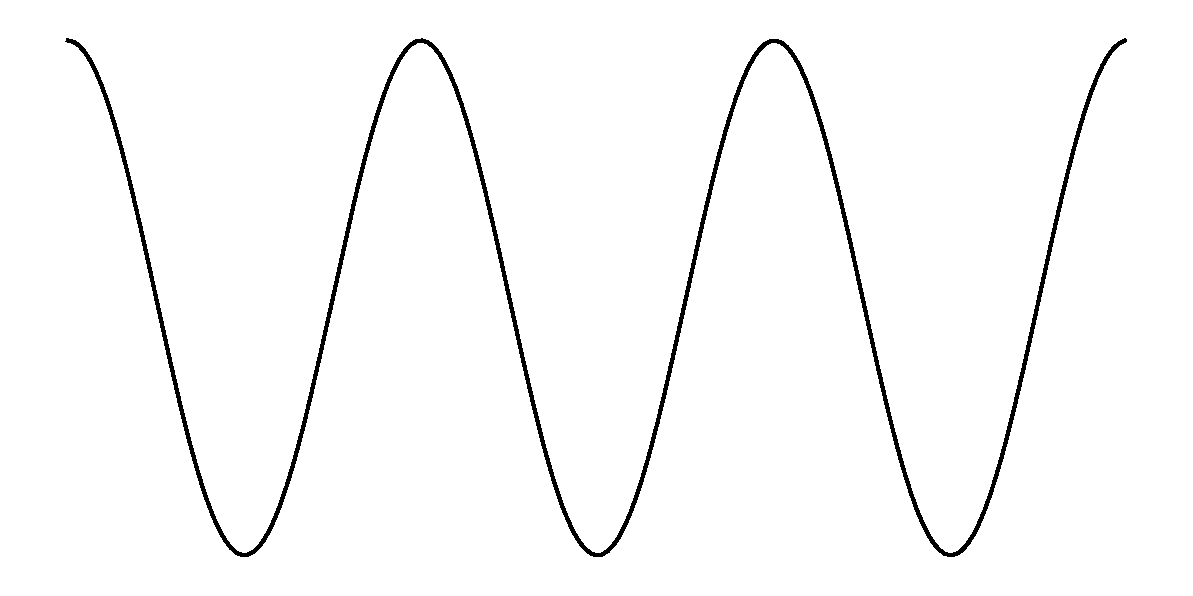
\includegraphics[width=\textwidth]
{figures/a_basic_wave.pdf}}
\caption{\label{fig:my-label} A Simple Wave}
\end{figure}

\subsection{Blue Whales Yelling - Amplitude}
What makes music such a great place to start is the fact that the human mind is already so used to picking out different sections, rhythms, and instruments - an activity quite similar to what we want to do with our frog chorus. When you go to a concert you can distinguish the vocals from the percussion, and the harmony from the melody. But, depending on the kind of concert it can be much more difficult picking out what your friends are trying to say when you're already having to yell to hear yourself. And by the end you'll all be speaking in muted whispers no matter how loud you try to speak because you'll have lost your voices half way through the performance. This contrast, conveniently, is our first and simplest discriminator of sound - volume. As you raise your voice the volume of the sound that you are producing increases. The fact that you can barely hear each other speaks to the enormous volume of sound coming from the stage. So how is this represented in our wave? Volume is determined by the height of our wave - the farther the undulation has to go between each peak and valley the louder the sound is. This height is referred to as the \textbf{amplitude} and to get a sense of just how variable amplitude can be let's bring a blue whale to the concert.

Blue whales are the largest animals to have ever lived. Rather unsurprisingly then, they can be rather loud. How loud? Well let's just say that blue whales would have no trouble hearing each other at a rock concert. In fact they may instead draw the ire of their fellow concert goers as they drown out the music with their voices. The typical sound level at a rock concert is around 110 decibels (dB) \cite{chris}. Blue whales on the other hand have been recorded at up to 180 dB \cite{zcormier}. This difference is actually far more ridiculous than it first seems because of what a decibel actually is. When a decibel measurement increases by 10 it means the sound is around 3 \textit{times} louder. All to say that if our blue whales raised their voices, their chatter could get up to 21 times louder than the rock concert! Quite rude. Graphing this out in Figure 2 we can see that the amplitude of the blue whales yelling at one another (dashed line) is so large in comparison to the amplitude of the rock concert (solid line) that the rock concert's sound barely looks like a wave at all. Pretty incredible.

\begin{figure}[!htb]
\center{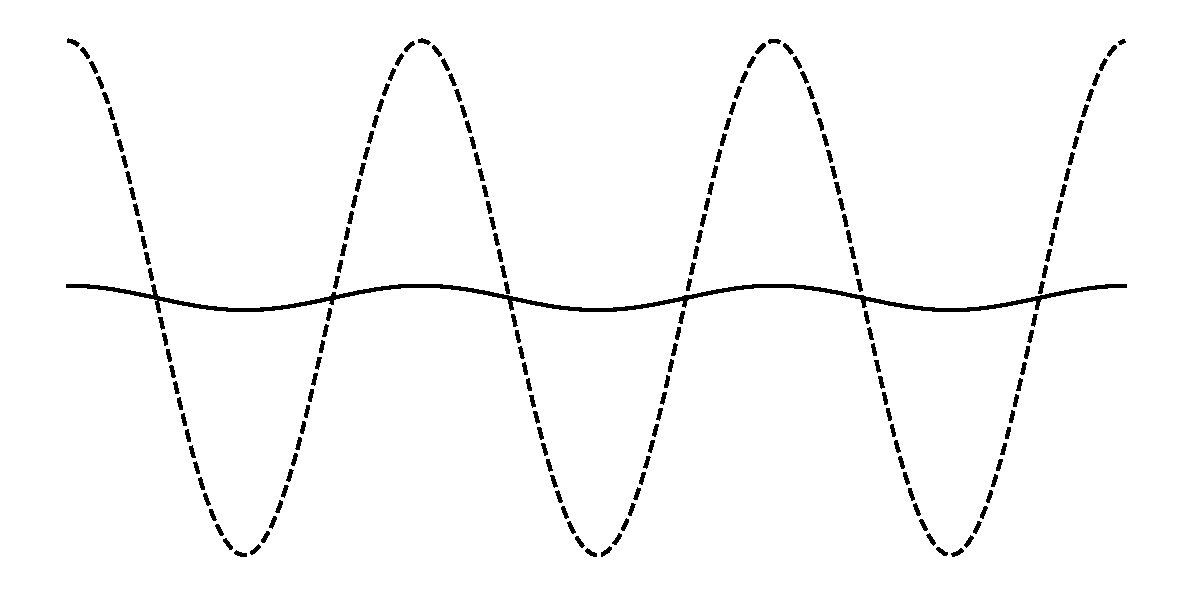
\includegraphics[width=\textwidth]
{figures/blue_whale_comparison.pdf}}
\caption{\label{fig:my-label} Blue Whale v. Rock Concert}
\end{figure}

\subsection{To Tune or Not to Tune - Pitch}
Okay, so amplitude is one way to distinguish one wave from another - what's up next? Well let's stop worrying about hearing our friends for a moment and turn back to the music. Remember how we said it's pretty easy for our brains to distinguish the vocalists from, say, the bass? Well there's a good reason for that - pitch. Pitch is how high or low a sound sounds. When that bass is rumbling all through your body you're experiencing a sound with a very low pitch. On the other hand when the singer hits that high note with a full crescendo that's a sound with an exhilarating high pitch. How does pitch show up in our wave? Well in contrast to amplitude - which was how high our waves got - pitch is all about how wide they are. The distance from one peak to the next is called the \textbf{wavelength} and the larger that distance is the lower the pitch of the sound. Pitch however is rarely measured in wavelengths. Instead the standard measurement used is something called Hertz (Hz). Hertz is a unit of \textbf{frequency} and frequency is simply the number of complete oscillations (peaks and troughs) per unit time. So, for example, when you hear that orchestras tune to A440 that 440 is specifically 440 Hz. Frequency and wavelength are interchangeable and tied together by a simple formula. Using the fact that we know the speed of sound $c$, if $w$ is the wavelength and $k$ is the frequency then the conversion is simply:

\begin{equation}
w = c/k
\end{equation}

So for example, if the speed of sound is 343 meters per second (m/s) then the wavelength of A440 is $343/440\approx0.78m$ or just over 2.5 feet. In comparison the highest note on a typical piano is at 7900 Hz \cite{wikipiano} which corresponds to a \textit{much} smaller wavelength ($343/7900=0.04m$). Figure 3 shows a comparison between the two with the solid line being A440 and the dashed line (which has a very very quick wiggle) being the highest note on a typical piano. Indeed the higher note has such a small wavelength it's becoming hard to see that it's a wave at all.

\begin{figure}[!htb]
\center{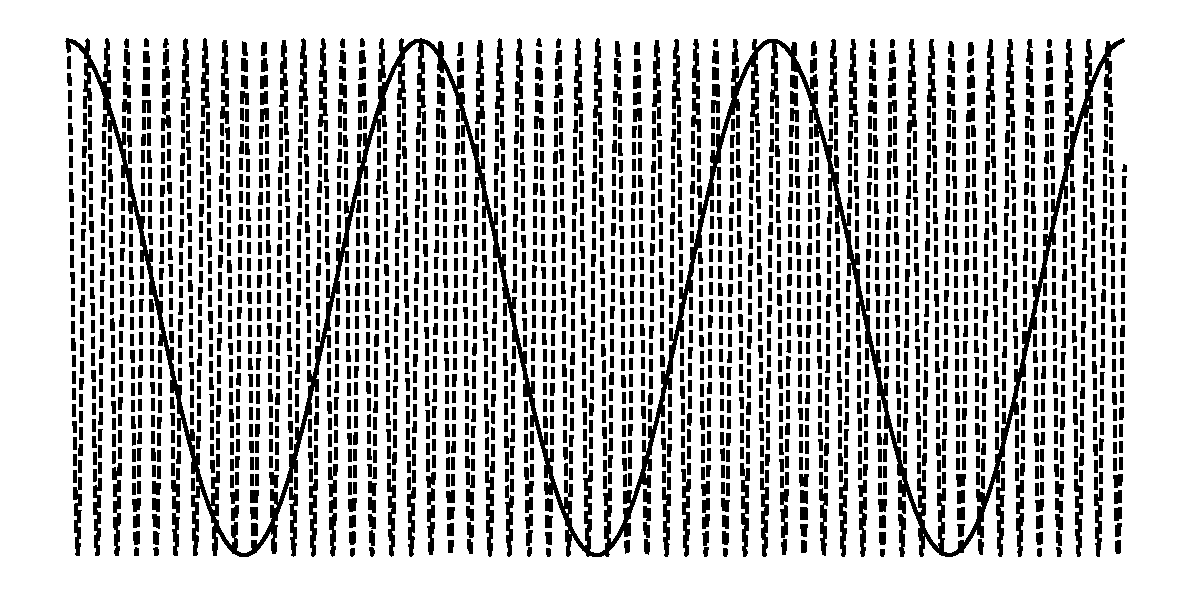
\includegraphics[width=\textwidth]
{figures/a440.pdf}}
\caption{\label{fig:my-label} A440 v. The Highest Note on a Piano}
\end{figure}

\subsection{The Quality of Sound - Superposition}
Now while pitch can certainly explain how we can tell the bass and the vocalist apart, how about sounds that are in the same range of pitch? For example a piano and our vocalist can both end up in in the same range of pitches and yet you'll still be able to tell them apart. What's going on here? Well, so far we've been oversimplifying things a lot. Remember how I said our picture of wave was the simplest picture possible? Well one of the ways in which it's super simple is that it's only got a single wavelength in it. In other words it has a single tone. Most sounds are not like this and are instead the composition of many wavelengths. This layering of wavelengths is called \textit{superposition} and it's best illustrated by an example. 

All sounds "begin" with a fundamental frequency - the lowest pitch in the sound. So let's begin with our simplest wave as the fundamental frequency (Fig 4.).

\begin{figure}[!htb]
\center{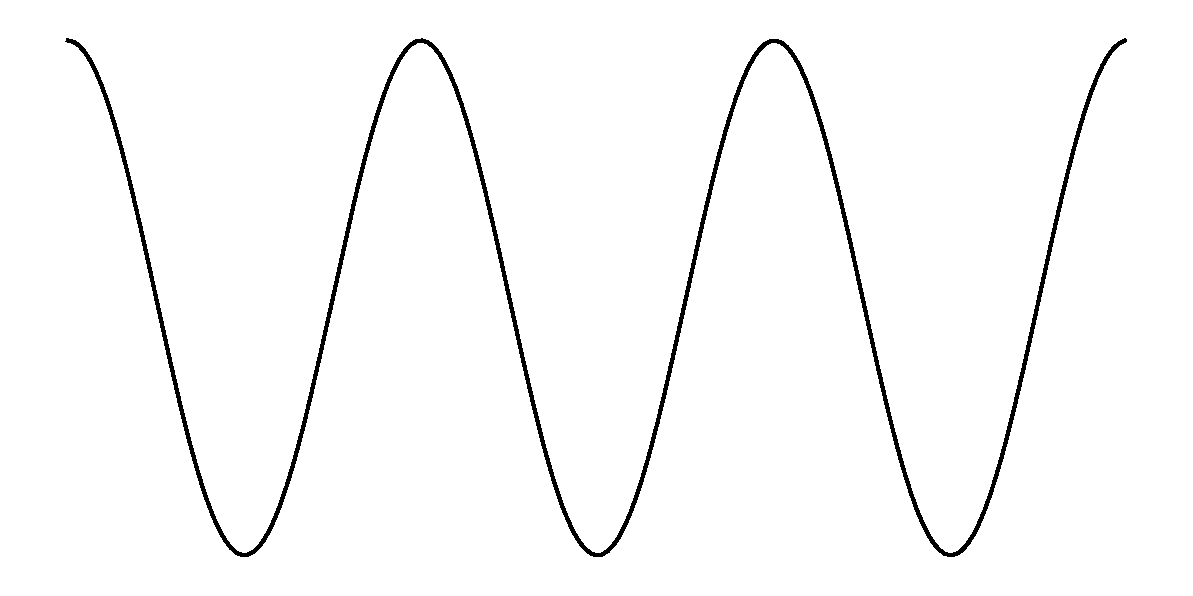
\includegraphics[width=\textwidth]
{figures/super1.pdf}}
\caption{\label{fig:my-label} Fundamental Frequency}
\end{figure}

With our fundamental frequency in place, let's add in our first higher frequency. Note that when superimposing waves, not only can their frequencies be different, but their amplitudes can be different as well (and almost always are). So to illustrate this we'll superimpose a wave with half the wavelength and half the amplitude on top of our fundamental frequency. Figure 5 shows both the two base waves (dashed) and the resulting superimposed wave (solid).

\begin{figure}[!htb]
\center{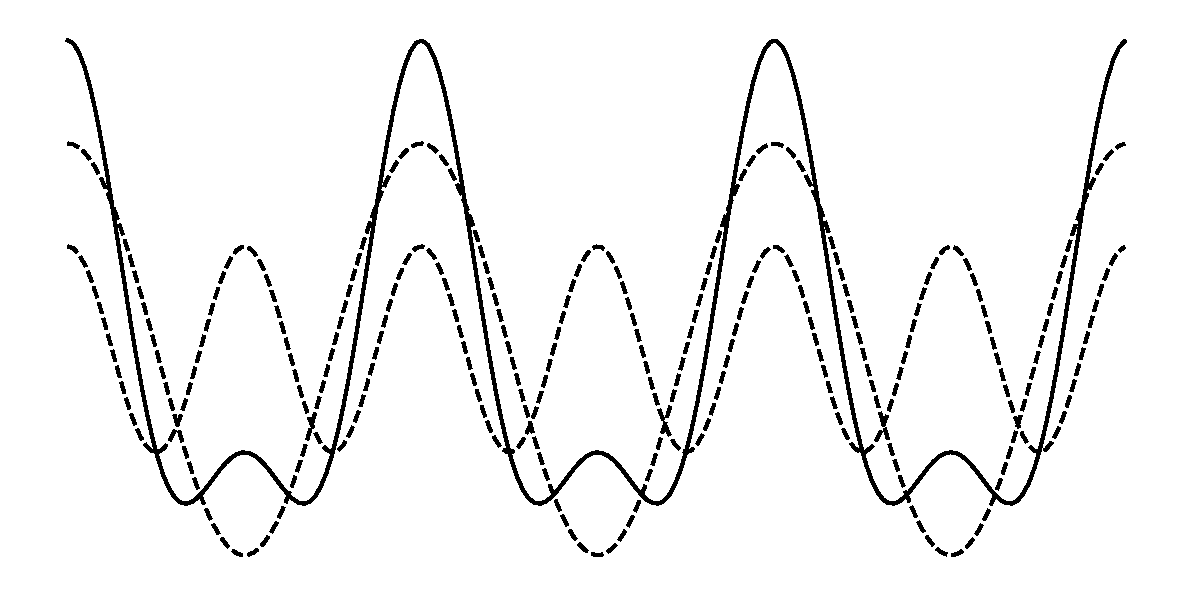
\includegraphics[width=\textwidth]
{figures/super2.pdf}}
\caption{\label{fig:my-label} Super Imposing Two Waves}
\end{figure}

Pretty wild right? (I find these kinds of waves starting looking really interesting and honestly kind of beautiful) 

Alright, let's add one more frequency in, this time with one quarter the wavelength and equal amplitude in comparison to our fundamental frequency (Fig. 6). 

\begin{figure}[!htb]
\center{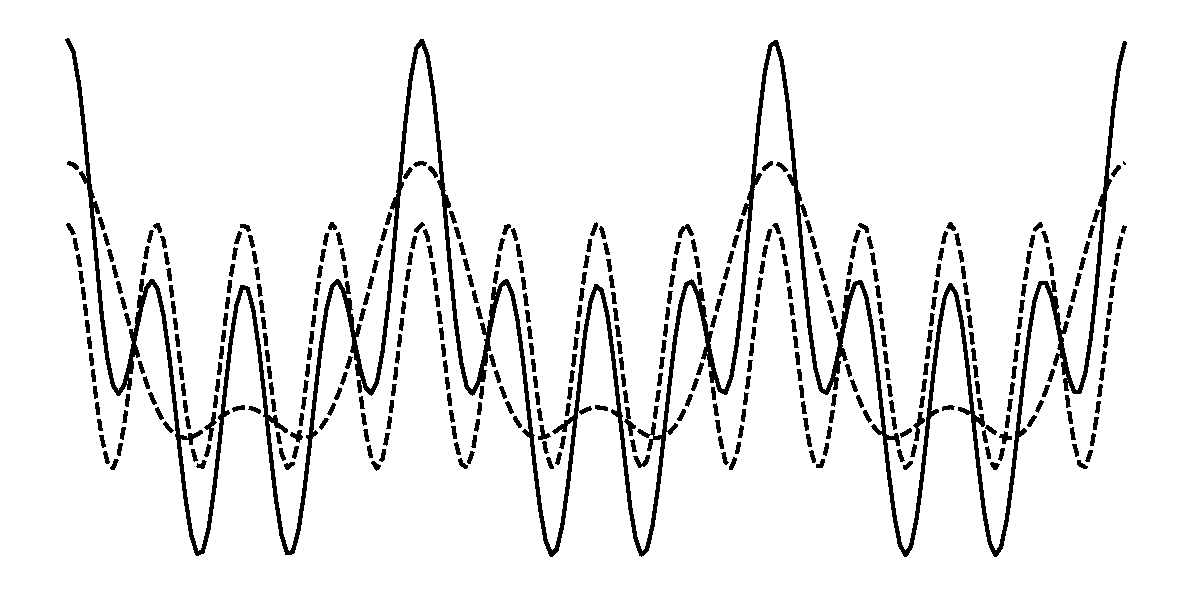
\includegraphics[width=\textwidth]
{figures/super3.pdf}}
\caption{\label{fig:my-label} Three Frequencies}
\end{figure}

Alright, while this is cool and nerdy and all, how does this relate back to distinguishing a piano from a vocalist? Well, when you play a note on any instrument the resulting sound is the superposition of whole load of different frequencies grounded on top of that fundamental frequency. What makes each instrument sound different, even when they're playing similar notes, is the fact that their particular mix of frequencies and amplitudes are each different. The combination particular to one instrument is what gives it its particular sound. In fact, for a trained ear, these differences can even allow you to identify one instrument from another. For example a piano with higher amplitudes at higher frequencies literally sounds brighter than one with muted amplitudes at higher frequencies. Superposition then, and the particular mix of frequencies and amplitudes that make up a specific sound, is yet another tool in our tool box of ways to distinguish one sound source from another. 

\subsection{Vanishing Act - Phase}
So we've now got amplitude, wavelength, and superposition which brings us to the final component we can use in describing our waves. This one is probably the most abstract and weird of the bunch, but it's one we're going to take advantage of a \textit{lot} and its name is \textbf{phase}. 

Thus far we've been looking at all of these waves as being in one spot in our graph. But there's no reason why we can't start shifting them from left to right (Fig 7.). This shifting is phase.

\begin{figure}[!htb]
\center{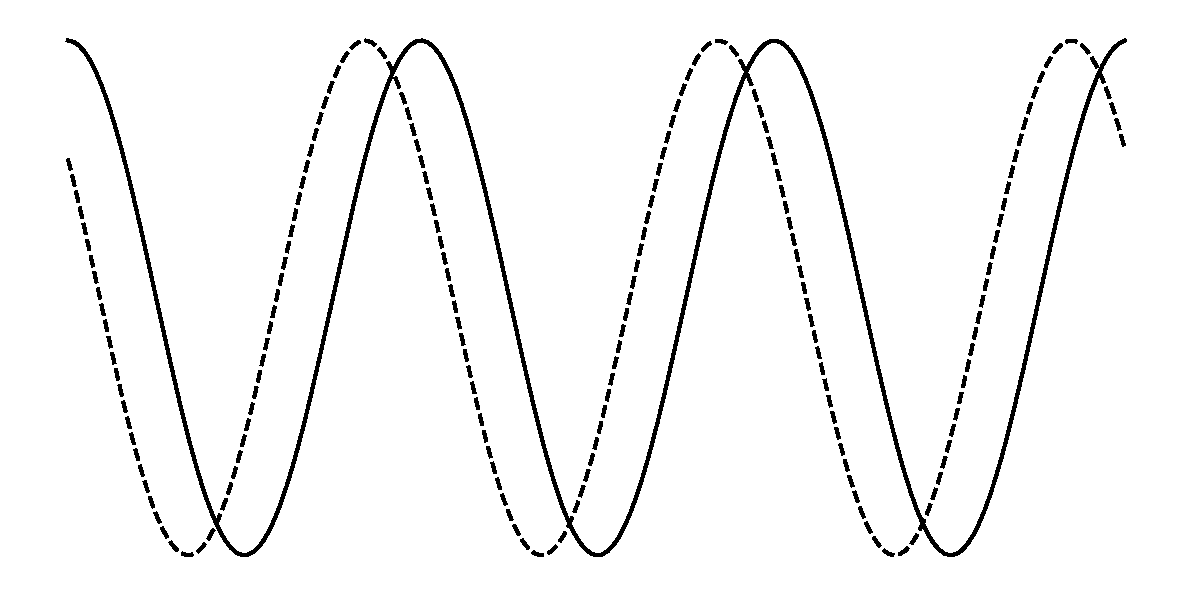
\includegraphics[width=\textwidth]
{figures/phase.pdf}}
\caption{\label{fig:my-label} Two Waves with Different Phases}
\end{figure}

What gets really weird (and where we start to see the power of phase) is when we superimpose two waves with the same wavelength but different phases. 

Figure 8 shows the super position of the two waves from Figure 7. Note how because the waves are nearly in sync (peaks match with peaks and troughs match with troughs) they add together to create a wave with much higher amplitude. This is known as \textbf{constructive interference}.

\begin{figure}[!htb]
\center{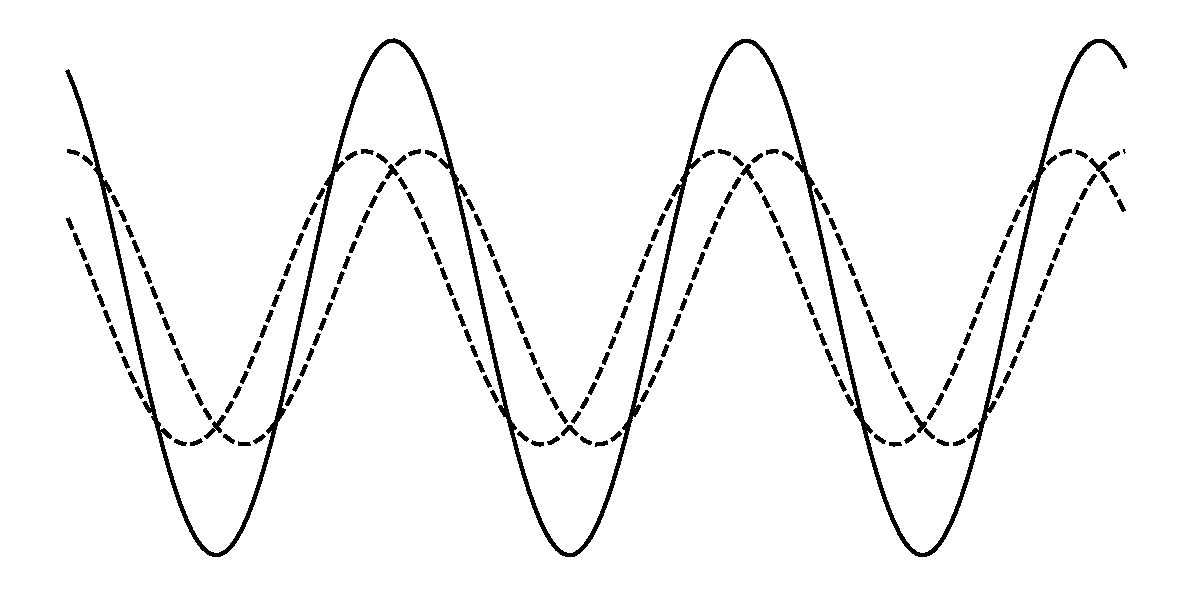
\includegraphics[width=\textwidth]
{figures/phasesuper1.pdf}}
\caption{\label{fig:my-label} Constructive Interference}
\end{figure}

On the other hand, Figure 9 shows the superposition of two waves that are nearly out of sync (peaks at troughs and troughs at peaks). Note how in this case the resulting wave is much smaller than either of the constituents - this is \textbf{destructive interference}.

\begin{figure}[!htb]
\center{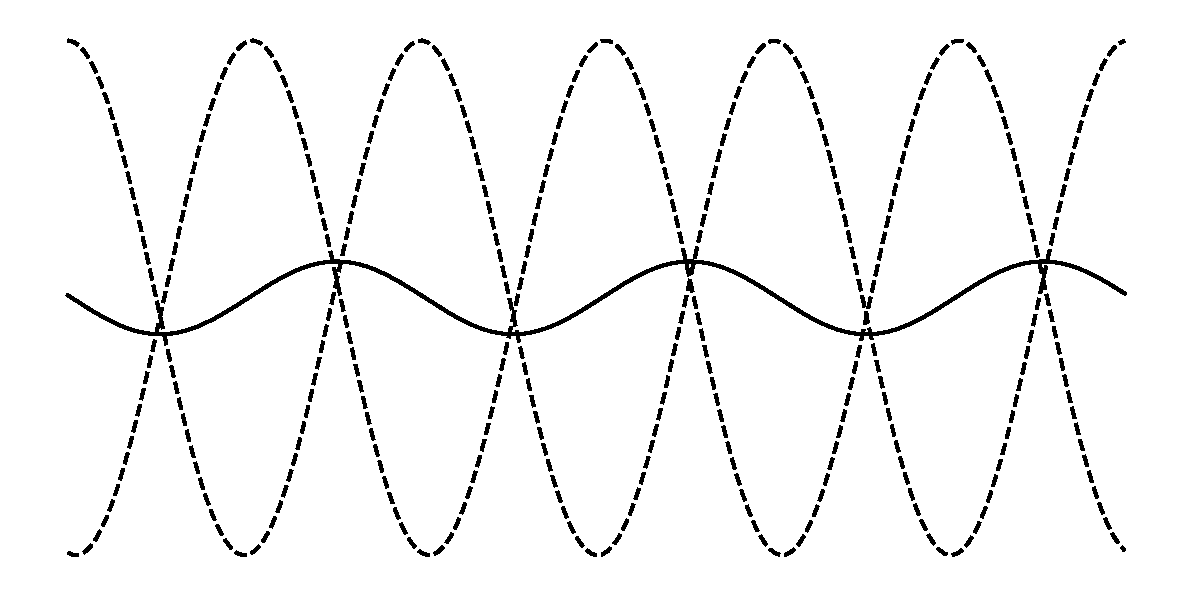
\includegraphics[width=\textwidth]
{figures/phasesuper2.pdf}}
\caption{\label{fig:my-label} Destructive Interference}
\end{figure}


What's really weird is that if you get the two waves to be exactly out of sync, the resulting superposition \textit{vanishes}! What does this mean physically? It means that the sound itself disappears! Yep, that's right, if two sound sources have just the right phase difference you'll suddenly no longer hear them even though the underlying sounds are there. Absolutely wild right? Well it turns out that this odd mathematical feature helps your brain figure out where sound is coming from.

Suppose a sound is coming directly from your right. That sound will obviously hit your right ear first. A very very short time later the same wave will hit your left ear, but at that point the undulation at your right ear will have changed (because the wave is constantly, well, waving). This difference in what your right and left ear are receiving is equivalent to the phase shift we were just talking about. Now suppose the sound is coming from directly in front of you. In this case the sound hits both ears at the same time because the distance to each ear is the same. This means there is no phase difference. What these two examples show is that as a sound source moves around your head the phase difference between your two ears changes. And your brain can use these differences to help you pick out where the sound is coming from! \cite{wikilocalization}. Pretty amazing, right? This happens to be the simplest version of a very cool technology called a \textbf{phased array} - something we'll be diving into detail next. But before we get to that we need to pull together all the tools we've gathered up so far and formalize them mathematically because phased arrays get pretty technical. So let's step back and do just that.

\subsection{Sums and Summaries - Mathematical Formalization}
Alright, so we've got all our pieces:
\begin{itemize}
\item \textbf{Amplitude:} The height of a wave, representing volume.
\item \textbf{Wavelength (or Frequency):} The width of a wave, representing pitch.
\item \textbf{Superposition:} The particular mix of amplitudes and frequencies that make up a sound.
\item \textbf{Phase:} An abstract sense of the "position" of a wave that leads to destructive or constructive interference.
\end{itemize}

How do we tie them all together mathematically? Well our simplest of waves is described by the following formula:
\begin{equation}
y=a e^{i\psi}e^{ikx}
\end{equation}
$e=2.71828$ is a mathematical constant known as Euler's number. $i=\sqrt{-1}$ is the imaginary number. $a$ is our amplitude. $k=2\pi/w$ where $w$ is our wavelength. Last but certainly not least, $\psi$ (pronounced like \textit{sigh}) is our phase. 

That then gets us three out of our four. So what about superposition? Well remember superposition is just adding many simple waves together, so we can do just that: 
\begin{equation}
y = a_1 e^{i\psi_1}e^{ik_1x} + a_2 e^{i\psi_2}e^{ik_2x} + ... + a_N e^{i\psi_N}e^{ik_Nx}
\end{equation}
Now writing out all these terms all of the time is going to get really burdensome, so we're going to take advantage of a little bit of mathematical notation that you may or may not be familiar with - the sum $\Sigma$. 

If you're not familiar with this notation, let's demonstrate with a simpler example. Suppose that you were adding the numbers 1 through 100. Without $\Sigma$ you would write:
\begin{equation}
1 + 2 + 3 + ... + 100
\end{equation}
With $\Sigma$ this same expression becomes:
\begin{equation}
\sum_{n=1}^{100}n
\end{equation}
which reads as - "add together all the $n$ (the thing to the right of the $\Sigma$) where $n$ starts at 1 (expression below the $\Sigma$) and goes all the way to 100 (number above the $\Sigma$)". I appreciate that this is probably pretty abstract and a little mind bending if this is your first time seeing it, but as we dive further into our little adventure you'll see just how useful this one bit of notation is. Alright, back to our waves.

Our superposition of waves goes from looking like this
\begin{equation}
y = a_1 e^{i\psi_1}e^{ik_1x} + a_2 e^{i\psi_2}e^{ik_2x} + ... + a_N e^{i\psi_N}e^{ik_Nx}
\end{equation}
to this:
\begin{equation}
y = \sum_{n=1}^{N}a_n e^{i\psi_n}e^{ik_nx}
\end{equation}
which is far neater and, as will become clear later, far easier to work with. 

That's it then! We've got our equation for a wave and are clear on the various components that make one sound different from another. With these tools in hand let's go and look at an absolutely incredible (and mathematically beautiful) technology for sound localization based on nothing more than our two ears - the phased array. 

\newpage
\section{To Phase Array}
The one where we get into the math of phased arrays
\section{How Tall is A-flat?}
The one where we show how difficult sound is to work with
\section{The Fourth Dimension}
The one where we explain how we're going to get around sound's limitations
\section{A Frog in a Sound-stack}
The one where we explain the approach to the unsolved problem
\section{The Descent of Math}
The one where we work out the ML math
\section{Divergent Degenerates}
The one where we deal with some technical issues of our gradient
\section{We Did a Thing}
The one where we bring it all together
\section{What's Going On?}
The one where we reflect on what we achieved
\newpage
\bibliographystyle{plain}
\bibliography{reference}

\end{document}